\section{Compressed Sensing (CS)}
%=========================================================================================

\begin{frame}{Compressed Sensing}

	\begin{columns}
		\begin{column}{0.45\textwidth}
			\begin{figure}
				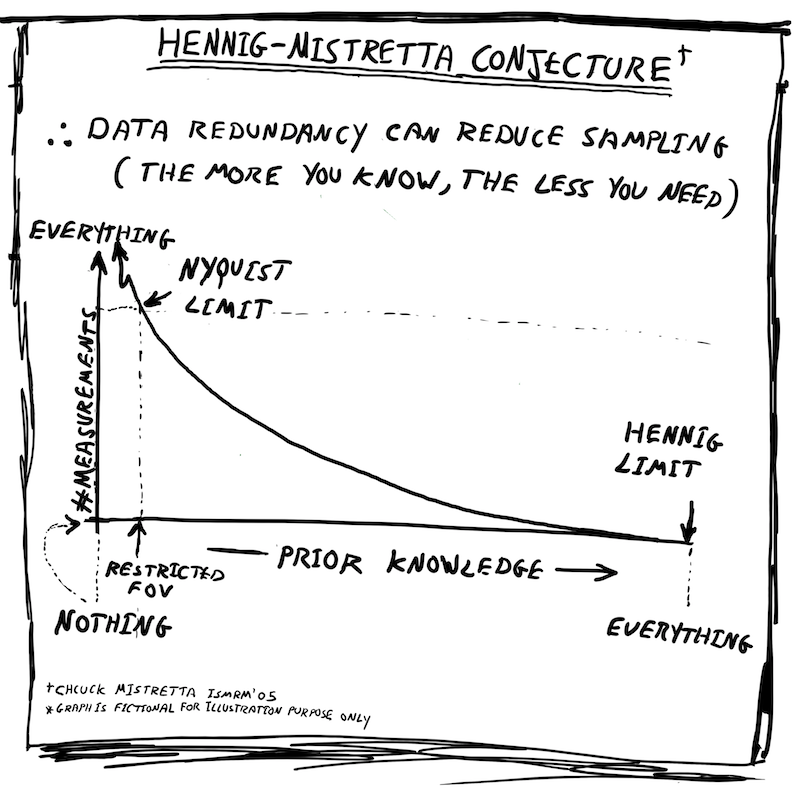
\includegraphics[width=\columnwidth]{fig/comics_02.png}
			\end{figure}
		\end{column}
	
		\begin{column}{0.55\textwidth}
			\begin{itemize}
				\item Candes EJ, Romberg JK, Tao T. Stable signal recovery from incomplete and inaccurate measurements. \textit{Commun Pure Appl Math} (2006).
				\vspace{0.5em}
				\item Lustig M, Dohono D, Pauly JM. Sparse MRI: The application of compressed sensing for rapid MR imaging. \textit{Magn Reson Med} (2007).
				\vspace{0.5em}
				\item Block KT, Uecker M, Frahm J. Undersampled radial MRI with multiple coils. Iterative image reconstruction using a total variation constraint. \textit{Magn Reson Med} (2007).
				\vspace{0.5em}
				\item Comics from \url{http://people.eecs.berkeley.edu/~mlustig/comics1.html}
			\end{itemize}
			\vfill
		\end{column}
	\end{columns}
\end{frame}


\begin{frame}{What is Nyquist Limit?}
	
	\begin{block}{Nyquist Sampling Requirement}
		{\large
		Given an imaging field-of-view (FOV), the sampling in $k$-space must satisfy
		\begin{equation}
			\Delta k \leq 1/\mathrm{FOV}
		\end{equation}}
	\end{block}
	
	\begin{figure}
		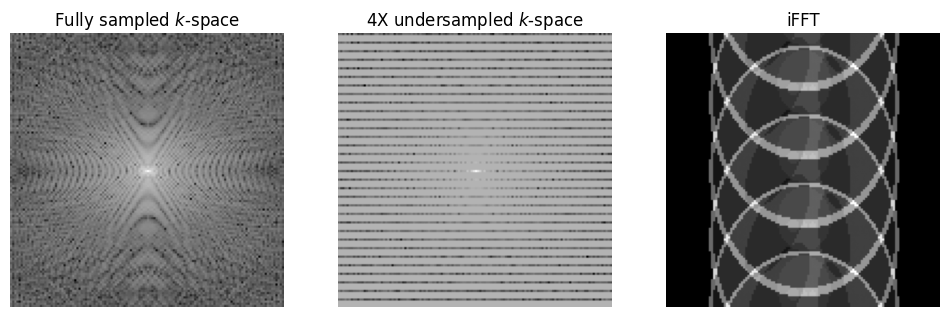
\includegraphics[width=0.9\textwidth]{fig/Nyquist.png}
	\end{figure}
	
\end{frame}


\begin{frame}{How Compressed Sensing Goes Beyond Nyquist?}

	\begin{columns}
		\begin{column}{0.45\textwidth}<1->
			\begin{figure}
				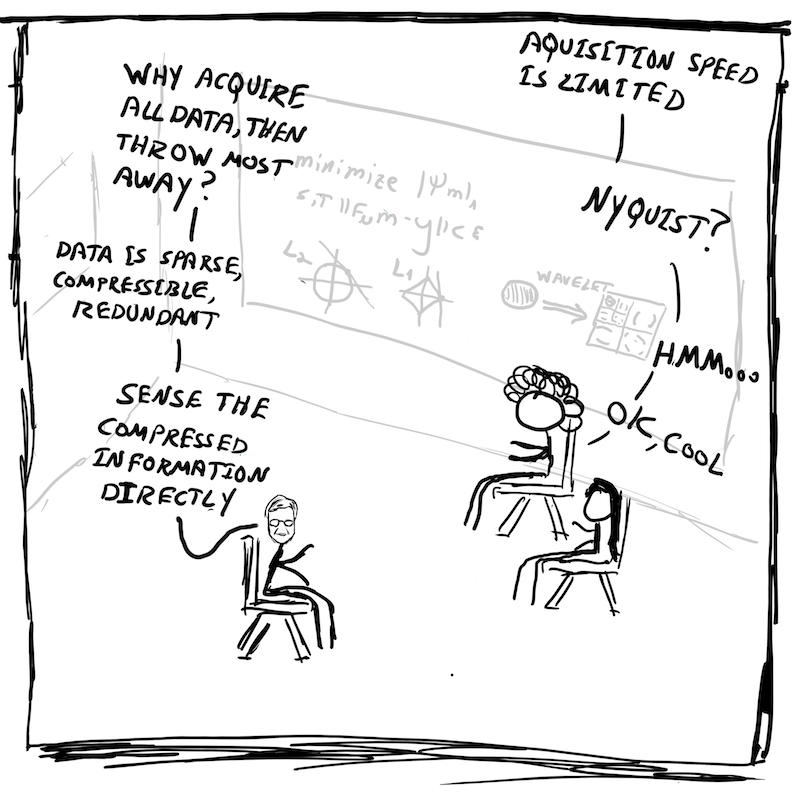
\includegraphics[width=\columnwidth]{fig/comics_04.png}
			\end{figure}
		\end{column}
		\begin{column}{0.45\textwidth}<2->
			\begin{figure}
				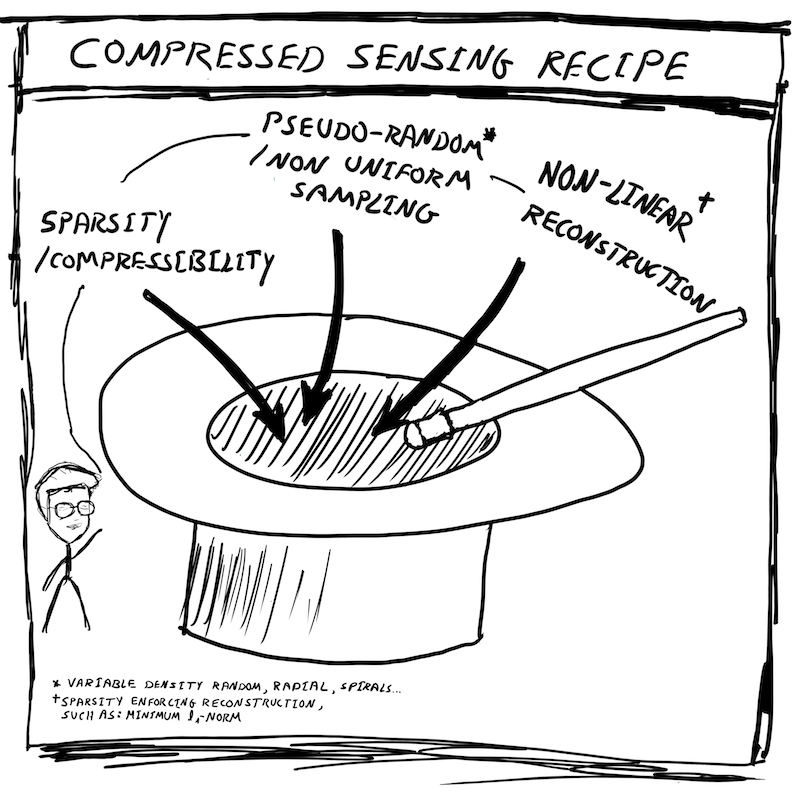
\includegraphics[width=\columnwidth]{fig/comics_05.png}
			\end{figure}
		\end{column}
	\end{columns}
\end{frame}


\begin{frame}{Before Compressed Sensing: Parallel Imaging as SENSE \footnote{Pruessmann KP, Weiger M, Scheidegger MB, Boesiger P. SENSE: sensitivity encoding for fast MRI. \textit{Magn Reson Med} (1999).}}
	
	\begin{figure}
		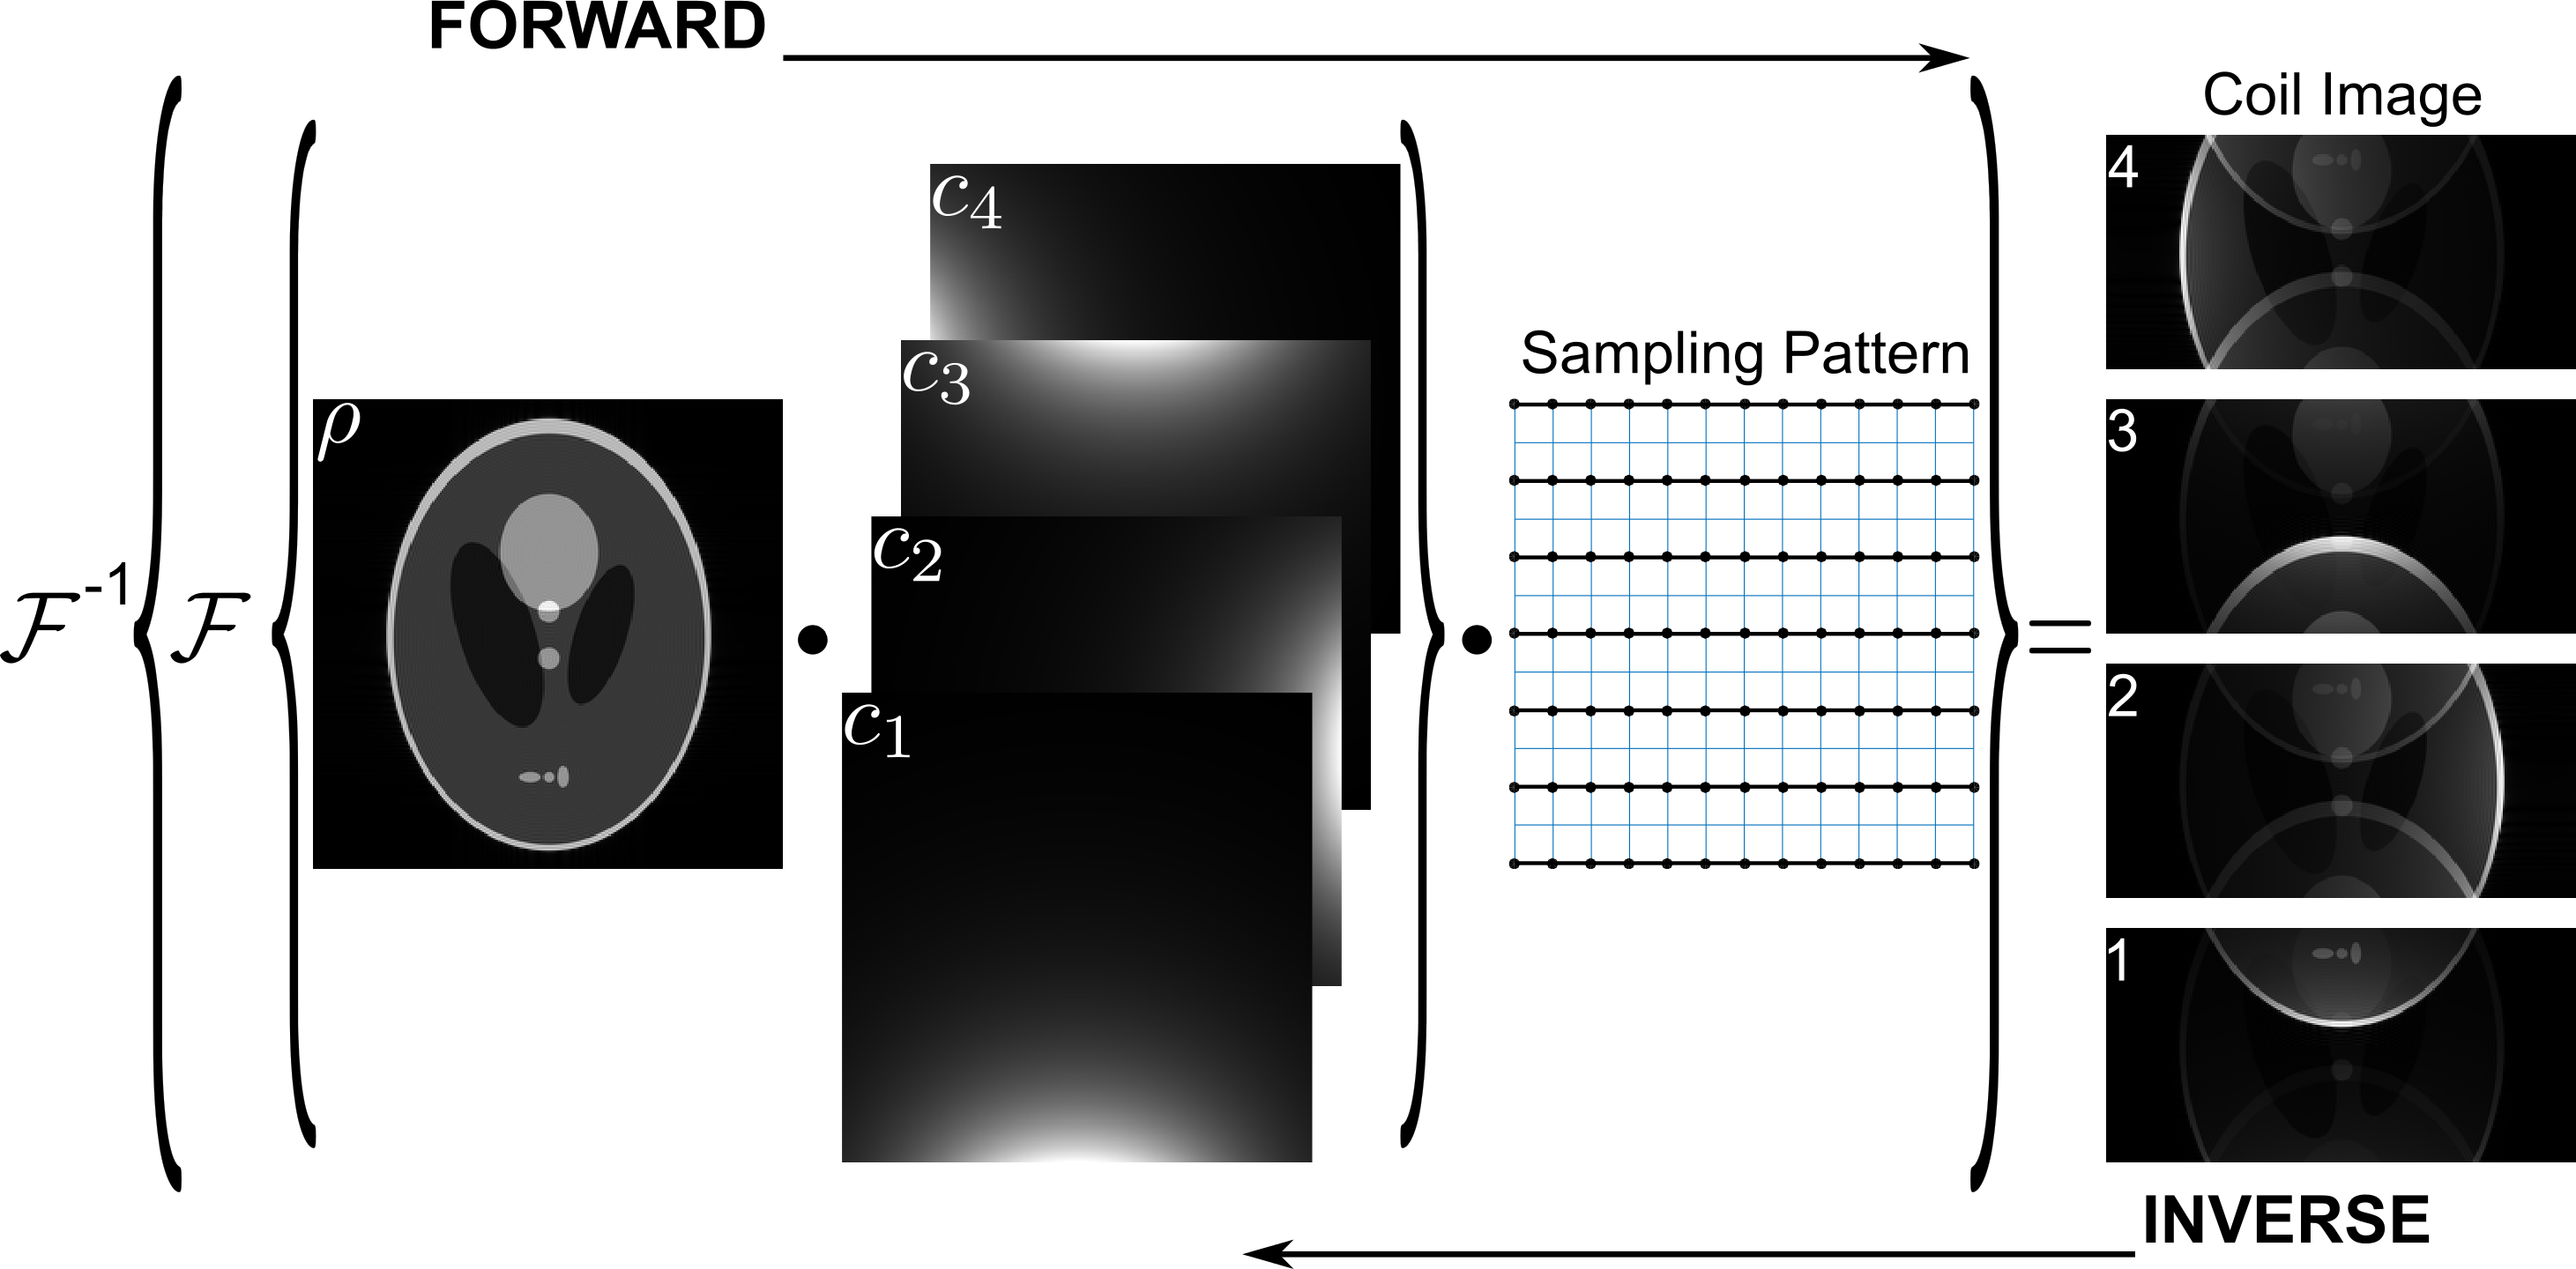
\includegraphics[width=0.8\textwidth]{fig/mri-pi.png}
	\end{figure}
	
\end{frame}


\begin{frame}{Parallel Imaging as SENSE: Solving a Linear Inverse Problem}
	
	Objective function:
	
	\begin{equation}
		\mathrm{argmin}_x \lVert y -  \mathcal{P} \mathcal{F} \mathcal{S} x \rVert_2^2
	\end{equation}

	\vfill

	\begin{itemize}
		\item Solver: gradient descent, or conjugate gradient, or ADAM, ...
		\vspace{1em}
		\item Data update via gradient method, e.g.~FISTA \footnote{Beck A, Teboulle M. A fast iterative shrinkage-thresholding algorithm for linear inverse problems. \textit{SIAM J Imaging Sciences} (2009).}: \\
		\vspace{1em}
		\hspace{5em} $x^{(t+1)} = x^{(t)} + \alpha \cdot \mathcal{S}^H \mathcal{F}^{-1} \mathcal{P}^{H} (y - \mathcal{P} \mathcal{F} \mathcal{S} x^{(t)})$
	\end{itemize}

\end{frame}


\begin{frame}{What is Linear Inverse Problem and What is Gradient?}
	
	Objective function:
	
	\begin{equation}
		\mathrm{argmin}_x \lVert 2 - x \rVert_2^2
	\end{equation}

	\vfill

	Given initial guess $x_\mathrm{prev} = 0$ and learning rate $\alpha = 0.1$,
	
	\begin{table}
		\centering
		\begin{tabular}{p{0.1\textwidth} p{0.25\textwidth} p{0.25\textwidth} p{0.25\textwidth}}
			\toprule
			Iteration & $x_\mathrm{prev}$ & $\mathrm{grad} = 2 * (2 - x)$ & $x_\mathrm{curr} = x_\mathrm{prev} + \alpha * \mathrm{grad}$ \\
			\midrule
			0 & 0 & 4 & 0.4 \\
			1 & 0.4 & 3.2 & 0.72 \\
			\vdots & \vdots & \vdots & \vdots \\
			47 & 1.9999 & 0.0001 & 2 \\
			\bottomrule
		\end{tabular}
	\end{table}
	
\end{frame}


\begin{frame}{What is Linear Inverse Problem and What is Gradient?}
	
	\begin{figure}
		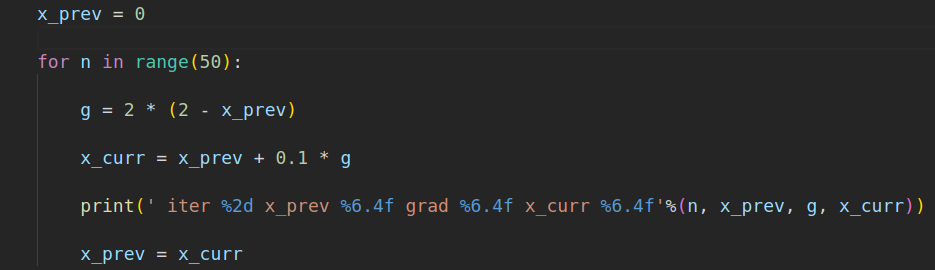
\includegraphics[width=\textwidth]{fig/gradient.png}
	\end{figure}
	
\end{frame}


\begin{frame}{Inverse Problems can Become Under-determined / Ill-posed}
	Objective function:
	
	\begin{equation}
		\mathrm{argmin}_{x_1, x_2} \lVert 2 - x_1 - x_2 \rVert_2^2
	\end{equation}

	\vfill
	
	\begin{itemize}
		\item <1-> You can't find an unique solution for this function.
		\vspace{1em}
		\item <2->..., however, when there is prior knowledge, e.g. \\
		\begin{equation}
			\mathrm{s.t.}~x_1 = x_2
		\end{equation}
	
		\item <3-> We can easily solve it, $x_1 = x_2 = 1$.
	\end{itemize}

\end{frame}


\begin{frame}{We can write this toy example in a matrix format}
	Objective function:
	
	\begin{equation}
		\mathrm{argmin}_{x_1, x_2} \lVert 2 - x_1 - x_2 \rVert_2^2
	\end{equation}

	\vspace{1em}
	
	It is equivalent to
	\begin{equation}
		\mathrm{argmin}_{\mathbf{x}} \lVert \mathbf{y} - \mathbf{A} \mathbf{x} \rVert_2^2
	\end{equation}
	\hspace{1em} where $\mathbf{x} = \begin{pmatrix}
		x_1 \\ x_1
	\end{pmatrix}$, $\mathbf{y} = \begin{pmatrix}
	2 \\ 2
	\end{pmatrix}$ and 
	$\mathbf{A} = \begin{pmatrix}
		1 & -1 \\
		1 & -1
	\end{pmatrix}$

	\vspace{3em}
	Does it look similar to the inverse problem in MRI?
	\begin{equation}
		\mathrm{argmin}_x \lVert y -  \mathcal{P} \mathcal{F} \mathcal{S} x \rVert_2^2
	\end{equation}
\end{frame}


\begin{frame}{Prior is the Game Changer in Compressed Sensing}
	\begin{itemize}
		\item <1-> Prof.~Dr.~Gary Golver from Stanford:\\
		"We eventually only need to measure one point in $k$-space!!!"
		\vspace{1em}
		\item <2->People like me:\\
		"What is going on here??? Is there anyone who would like to share their codes???"
		\vspace{1em}
		\item <3-> Prof.~Dr.~Mike Lustig from Berkeley:\\
		"Sparsifying transformation changes the game!!!"
		\begin{equation}
			\mathrm{argmin}_x \lVert y -  \mathcal{P} \mathcal{F} \mathcal{S} x \rVert_2^2 + \lambda \lVert \Phi x \rVert_1
		\end{equation}
		where $\Phi$ is wavelet transform, total variation, ...
	\end{itemize}
	
	
\end{frame}


\begin{frame}{How to Solve this Problem?}
	Objective function:

	\begin{equation}
		\mathrm{argmin}_x \lVert y -  \mathcal{P} \mathcal{F} \mathcal{S} x \rVert_2^2 + \lambda \lVert \Phi x \rVert_1
	\end{equation}

	\begin{itemize}
		\item the regularization term $\lambda \lVert \Phi x \rVert_1$ is not differentiable;
		\item soft thresholding $\mathcal{T}_\lambda(x) = (x - \lambda)_+ \mathrm{sign}(x)$
	\end{itemize}

	\begin{figure}
		\centering
		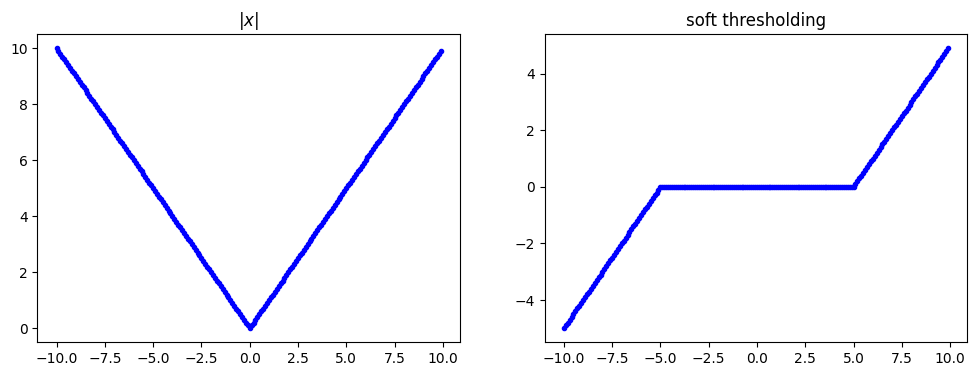
\includegraphics[width=0.8\textwidth]{fig/soft_thresh.png}
	\end{figure}

\end{frame}


\begin{frame}{Compressed Sensing: Iterative Soft Thresholding}
	\begin{enumerate}
		\item Gradient update:\\
		\hspace{4em} $x^{(t+1)} = x^{(t)} + \alpha \cdot \mathcal{S}^H \mathcal{F}^{-1} \mathcal{P}^{H} (y - \mathcal{P} \mathcal{F} \mathcal{S} x^{(t)})$
		\vspace{2em}
		\item Soft thresholding:\\
		\hspace{4em} $x^{(t+1)} = \Phi^{-1}\mathcal{T}_\lambda(\Phi x^{(t+1)})$
	\end{enumerate}

	\vspace{1em}
	\hrule
	\vspace{1em}
	
	\begin{itemize}
		\item This suffices when $\Phi$ is wavelet transform. 
		\item When you use total variation, you may need a more general solver such as ADAM.
	\end{itemize}

\end{frame}


\begin{frame}{What is Gradient Update in Parallel MRI? \footnote{Pruessmann KP, Weiger M, B\"ornert P, Boesiger P. Advances in sensitivity encoding with arbitrary $k$-space trajectories. \textit{Magn Reson Med} (2001).}}
	\begin{figure}
		\centering
		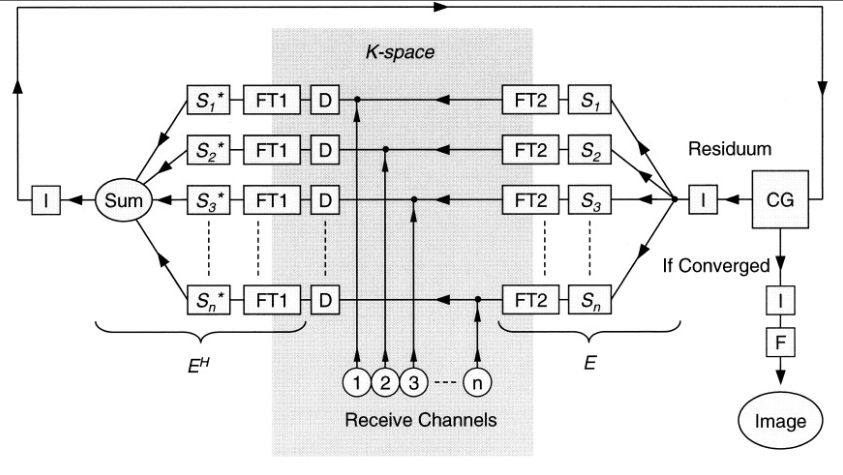
\includegraphics[width=0.75\textwidth]{fig/cgsense.png}
	\end{figure}
\end{frame}


\begin{frame}{Gradient Update in Parallel MRI: CG SENSE}
	
	\begin{itemize}
		\item density correction $D$:\\
		$D = 1 / d \mathbf{k}$, $\mathbf{k}$ is the relative density of the $k$-space sampling pattern at the position $\vec{k}$.
		\vspace{2em}
		\item this changes the system equation:\\
		$(E^H D E) \mathbf{v} = E^H D \mathbf{m}$
		\vspace{2em}
		\item <2-> this speeds up the iterative procedure in practice. However, mathematicians don't like it ...
		\vspace{1em}
		\item <3-> Exercise 1: run the gradient step many times without soft thresholding, are you able to get a similar reconstruction as the NUFFT reconstruction with density compensation?
		\vspace{1em}
		\item <4-> Exercise 2: try to tune the soft thresholding parameter, and show how it affects the reconstruction
		
	\end{itemize}
	
\end{frame}



\begin{frame}{It is not the end ...}
	\begin{itemize}
		\item Prof.~Dr.~Florian Knoll \footnote{Hammernik K, Klatzer T, Kobler E, Recht MP, Sodickson DK, Pock T, Knoll F. Learning a variational network for reconstruction of accelerated MRI data. \textit{Magn Reson Med} (2018).}:\\
		"Instead of hand-crafted sparsifying transform, neural network learns it!!!"
	\end{itemize}
\end{frame}
